
\documentclass[10pt]{beamer}
\usepackage{kotex}

\usepackage{framed}
\usepackage{graphicx}
%https://www.overleaf.com/learn/latex/Inserting_Images

\usepackage{amsmath}
%use dfrac
\usepackage{xcolor}

\usepackage{amsthm}
%\usepackage{tabl}
\usepackage{listings}
\definecolor{mGreen}{rgb}{0,0.6,0}
\definecolor{mGray}{rgb}{0.5,0.5,0.5}
\definecolor{mPurple}{rgb}{0.58,0,0.82}
\definecolor{backgroundColour}{rgb}{0.95,0.95,0.92}
%https://tex.stackexchange.com/questions/348651/c-code-to-add-in-the-document
\lstdefinestyle{CppStyle}{
    backgroundcolor=\color{backgroundColour},   
    commentstyle=\color{mGreen},
    keywordstyle=\color{magenta},
    numberstyle=\tiny\color{mGray},
    stringstyle=\color{mPurple},
    basicstyle=\footnotesize,
    breakatwhitespace=false,         
    breaklines=true,                 
    captionpos=b,                    
    keepspaces=true,                 
    numbers=left,                    
    numbersep=5pt,                  
    showspaces=false,                
    showstringspaces=false,
    showtabs=false,                  
    tabsize=2,
    language=C++
}

\usepackage{url}

\usepackage{etoolbox}
\AtBeginEnvironment{quote}{\singlespacing\small}


\usepackage{thmtools}
\usepackage{xcolor}
\declaretheoremstyle[% spaceabove=6pt,spacebelow=6pt, headfont=\color{MainColorOne}\sffamily\bfseries, notefont=\mdseries, notebraces={[}{]}, bodyfont=\normalfont,
headpunct={},
postheadspace=1em,
%qed=▣,
]{maintheorem}

\declaretheorem[%
name=정의,
style=maintheorem,
numberwithin=section, shaded={%bgcolor=MainColorThree!20,
margin=.5em}]{dfn}
% \begin{dfn}[]
% \end{dfn}

\setbeamertemplate{footline}[frame number]

\usetheme{CambridgeUS}


\title{inheritance}

\author{EUnS}

\begin{document}


\begin{frame}{}
    \maketitle
\end{frame}    

\begin{frame}{}
    \tableofcontents
\end{frame}   

\section{inheritance}


\begin{frame}[fragile]{기본적인 모습}
    \begin{lstlisting}[style = CppStyle]
    class sample
    {
    public:
    virtual ~sample();
    };
    class sampleInheritance : public sample
    {
    public:
    };
    \end{lstlisting}
\end{frame}    


\begin{frame}{상속}
    \begin{itemize}
        \item 상속하는쪽 : 부모(super) 클래스 받는쪽: 자식(sub) 클래스
        \item 큰범위의 클래스(ex 사람) 작은 범위의 단위(ex 학생)으로 쪼개질때 큰범위의 정보를 포함하고 작아짐으로서 세세해지는 정보 또한 들어갈때 상속을 씀 is a 관계(a student is a person)
        \item 외부에서는 부모 클래스의 public + 자식 클래스의 public을 쓸 수 있다.
        \item 상속 방식 
        \begin{itemize}
            \item public : 외부에서 접근하는것처럼 부모클래스의 private,protect에 직접적인 접근 할 수 없음
            \item protected : 상속만을 위해 존재하는 접근지정자이며 추가적인것은 찾아볼것.
            \item private : 추가적인것은 찾아볼것.
        \end{itemize}
        \item 일반적으로 public상속을 쓴다(나머지 두개는 본인도 써본적없음)
    \end{itemize}
\end{frame}



\begin{frame}[fragile]{생성자 소멸자 순서}
    \begin{itemize}
        \item 소멸자는 가상함수로 선언하여야한다.
        \item 부모생성자 - 자식 생성자 순으로 불린다.
        \item 자식 소멸자 - 부모 소멸자 순으로 불린다.
    \end{itemize}
\end{frame}    


\section{virtual function}

\begin{frame}[fragile]{가상함수(virtual function)}
    \begin{lstlisting}[style = CppStyle]
    class sample
    {
        public:
        virtual ~sample();
        virtual void f() { ; }
        virtual void g() { ; }
        };
    class sampleInheritance : public sample
    {
        public:
        void f() override
        { ; }
        void g() final { ; }
        };
    \end{lstlisting}
\end{frame}

\begin{frame}[fragile]{가상함수(virtual function)}
    \begin{itemize}
        \item 상속 받는 클래스는 부모 클래스의 함수를 덮어 쓸 수 있다. 자식 클래스에 맞게 메소드를 다시 짜는것 이를 override라 한다.
        \item override할 부모 클래스 메소드에 virtual을 붙인다. 자식클래스에는 붙여도되고 안붙여도 됨.
        \item c++ keyword : \href{https://youtu.be/JMw0F8FFe80}{\textcolor{blue}{참고}}
        \begin{itemize}
            \item  override : override받는 메소드에 붙일 수 있다. override keyword를 붙인 멤버 함수가 override된 멤버함수가 아닐경우에 에러를 뱉는다.
            \item  final : 이 멤버 함수를 override하지 않으려고할때 붙일 수 있다. 상속받은 클래스가 이 멤버 함수를 override하면 에러를 뱉는다
        \end{itemize}
    \end{itemize}
\end{frame}

\begin{frame}{가상함수 작동 방식}
    \begin{itemize}
        \item 가상함수를 사용시 virtual function table이 생성된다.
        \item 가상함수가 들어간 클래스의 각 인스턴스는 가상함수테이블(vftable)을 가르키는 포인터(virtual function pointer vptr : 4byte)를 가짐
        \item virtual 선언만하고 정의를 빼려면 virtual type function() $=0$;
    \end{itemize}s
\end{frame}


\begin{frame}[fragile]{메모리 구조}
    \begin{figure}[h!]
        %\centering
        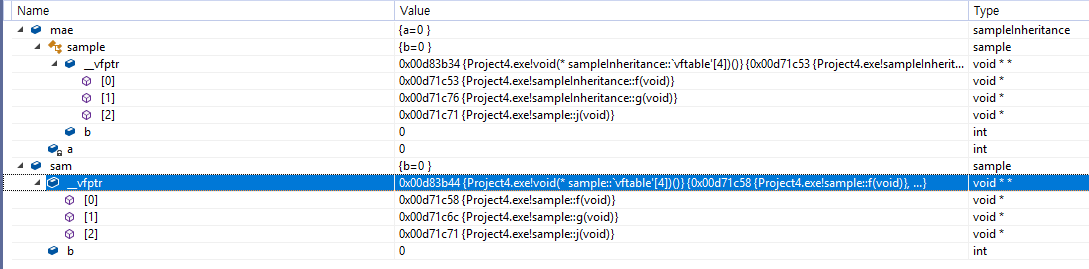
\includegraphics[scale=0.35]{virtual_table}
        \caption{vtbl}
    \end{figure}
\end{frame}    


\begin{frame}[fragile]{up casting}
    \begin{itemize}
        \item up casting : 부모 클래스의 자료형으로 자식 클래스를 가르키는것. 이때 소멸자를 가상함수로 선언하여야한다.
        \item down casting : up casting 된 부모 클래스의 포인터를 다시 자식 클래스 자료형 포인터로 가르키게 하는것.
    \end{itemize}
    \begin{lstlisting}[style = CppStyle]
        super* supPtr = new sub(); // up casting
        sub* subPtr1 =  (sub*)supPtr; // down casting1
        sub* subPtr2 = dynamic_cast<sub*>(supPtr); // down casting2
    \end{lstlisting}
\end{frame}

\section{etc}

\begin{frame}{찾아볼것}
    casting
    \begin{itemize}
        \item C sytle 
        \item $static\_cast<>()$ : \href{https://stackoverflow.com/questions/28002/regular-cast-vs-static-cast-vs-dynamic-cast}{\textcolor{blue}{참고}}
        \item $dynamic\_cast<>()$ 
        \item $reinterpret\_cast<>()$ \href{https://stackoverflow.com/questions/573294/when-to-use-reinterpret-cast}{\textcolor{blue}{참고}}
        \item $const\_cast<>()$ : 
    \end{itemize}
    $smart\_ptr$(C++11~)
    \begin{itemize}
        \item $unique\_ptr<>()$
        \item $shared\_ptr<>()$
        \item $weak\_ptr<>()$
    \end{itemize}
    enum class
\end{frame}



%https://stackoverflow.com/questions/3601602/what-are-rvalues-lvalues-xvalues-glvalues-and-prvalues

\begin{frame}{다중 상속(Multiple inheritance)}
    \begin{itemize}
        \item 직접 찾아볼것.
    \end{itemize}    
\end{frame}    



\begin{frame}{과제}
    \begin{itemize}
        \item 과제 1 : 코드 수정.
        \item 과제 0 : 상속 
        \item 과제 4 - 2 : 과제 1 + 과제 2
        \item 과제 5 - 2 : 팩토리 패턴, 싱글턴 패턴 적용하기 
    \end{itemize}
\end{frame}    

\end{document}

% 동적바운딩
% 업캐스팅 
%다운캐스팅
% RTTI
% dynamic_cast

% \begin{frame}{}
%     \href{}{\textcolor{blue}{참고}}
% \end{frame}        


% \begin{frame}{}
%     \begin{itemize}
%         \item 
%         \item 
%         \item 
%     \end{itemize}    
% \end{frame}

% \begin{frame}{}
%     \begin{figure}[h!]
%         %\centering
%         \includegraphics[scale=0.25]{}
%         \caption{}
%     \end{figure}
% \end{frame}


% \begin{lstlisting}[style = CppStyle]
%    
% \end{lstlisting}